% Created 2017-04-26 Wed 11:09
% Intended LaTeX compiler: pdflatex
\documentclass[10pt]{beamer}
\usepackage[utf8]{inputenc}
\usepackage[T1]{fontenc}
\usepackage{graphicx}
\usepackage{grffile}
\usepackage{longtable}
\usepackage{wrapfig}
\usepackage{rotating}
\usepackage[normalem]{ulem}
\usepackage{amsmath}
\usepackage{textcomp}
\usepackage{amssymb}
\usepackage{capt-of}
\usepackage{hyperref}
\logo{
\includegraphics[height=1.4cm,width=1.5cm]{RedHat-IsoLogo.jpg}}
\subtitle{Getting started with mailing list \& IRC}
\institute{Red Hat}
\setbeamertemplate{navigation symbols}[horizontal]
\usepackage{pxfonts}
\usepackage{hyperref}
\hypersetup{colorlinks=true, linkcolor=red, filecolor=magenta, urlcolor=cyan}
\urlstyle{same}
\usepackage{minted}
\usepackage[utf8]{inputenc}
\usepackage[english]{babel}
\setbeamertemplate{caption}[numbered]
\setbeamercovered{invisible}
\usetheme{Frankfurt}
\usecolortheme{}
\usefonttheme{serif}
\useinnertheme{rounded}
\useoutertheme{}
\author{Sachin}
\date{\today}
\title{Socializing with the community}
\usecolortheme[RGB={204,0,0}]{structure}%Red Hat
\hypersetup{
 pdfauthor={Sachin},
 pdftitle={Socializing with the community},
 pdfkeywords={},
 pdfsubject={Sample org beamer presentation},
 pdfcreator={Emacs 25.1.1 (Org mode 9.0.4)}, 
 pdflang={English}}
\begin{document}

\maketitle



\section{Intro}
\label{sec:orgd2ddf61}
\subsection{Intro}
\label{sec:org9e893a6}
\begin{frame}[label={sec:orgba37482}]{Question?}
\begin{itemize}
\item Whom do I ask questions?
\item Where do I ask questions?
\item How do I ask question?
\end{itemize}
\end{frame}

\begin{frame}[label={sec:orgf17f014}]{Motivation}
\begin{itemize}
\item You look for people with similar interests
\item With specific topic
\item \emph{Just want to be an observer}
\end{itemize}
\end{frame}

\begin{frame}[label={sec:org0a10c83}]{Mailing list?}
\begin{block}{Mailing list}
\emph{Send mail to multiple recipients}

\alert{**}
	 \url{https://www.redhat.com/mailman/listinfo/universityoutreach-pune}
\end{block}
\end{frame}

\begin{frame}[label={sec:org7edcab4}]{IRC?}
\begin{block}{\emph{Internet Relay Chat}}
\emph{Enable people to talk to each other via \alert{internet} exchanging
 textual messages}
\end{block}
\end{frame}


\begin{frame}[fragile,label={sec:orgb01ffde}]{IRC clients}
 \emph{**You need to install IRC client}

\begin{block}{\emph{Graphical}}
\begin{itemize}
\item \texttt{mIRC}
\item \texttt{hexchat}
\end{itemize}
\end{block}

\begin{block}{\emph{CommandLine}}
\begin{itemize}
\item \texttt{irssi}
\item \texttt{weechat}
\end{itemize}
\end{block}
\end{frame}

\begin{frame}[fragile,label={sec:orge8a01dd}]{IRC server}
 \emph{Listens to connections from IRC clients}


\begin{itemize}
\item \texttt{chat.freenode.net}
\item \texttt{irc.oftc.net}
\item \texttt{irc.gnome.org}
\end{itemize}
\end{frame}

\begin{frame}[fragile,label={sec:org2face9b}]{IRC server}
 \begin{minted}[]{sh}
/CONNECT chat.freenode.net
\end{minted}
\end{frame}


\begin{frame}[fragile,label={sec:org7a11e21}]{IRC channel}
 (\emph{\#kernelnewbies, \#vim, \#outreachy})


\begin{minted}[]{sh}
/JOIN #fedoraindia
/LEAVE #fedoraindia
\end{minted}
\end{frame}


\begin{frame}[fragile,label={sec:org7e92b5f}]{IRB Bot}
 \begin{block}{}
\texttt{psachin:} \emph{.weather pune}

\texttt{BB-8:} \emph{Pune, MH, IN: Sunny, 27 C (80 F), Humidity: 36\%}
\end{block}


\begin{block}{}
\texttt{psachin:} \emph{mrNobody++}

\texttt{BB-8:} \emph{mrNobody has 3 points of karma}
\end{block}


\begin{block}{}
\texttt{psachin:} \emph{psachin++}

\texttt{BB-8:} \emph{You cant give yourself karma}
\end{block}
\end{frame}


\begin{frame}[fragile,label={sec:org2b2336d}]{IRC on web(\texttt{http://webchat.freenode.net/})}
 \begin{center}
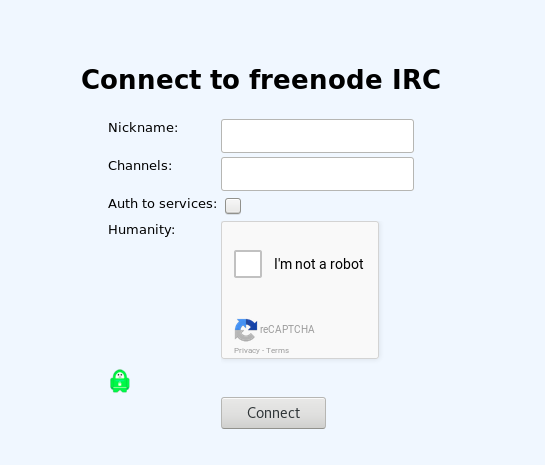
\includegraphics[width=.9\linewidth]{./webchat.freenode.png}
\end{center}
\end{frame}

\begin{frame}[fragile,label={sec:org55a1fef}]{IRC nick}
 \emph{Other users identify you by your \texttt{nick}. Avoid changing \texttt{nick}
once set}

\begin{block}{}
\texttt{guest2365:} /NICK psachin

\emph{You are now known as psachin}

\texttt{psachin:} \emph{Hello World}
\end{block}
\end{frame}

\section{etiquette}
\label{sec:orgeab0c8b}
\subsection{etiquette}
\label{sec:org509ca5c}
\begin{frame}[fragile,label={sec:orgf3d1d8b}]{NO naked pings}
 \begin{block}{}
\texttt{ircnewbie:} \emph{ping}

\texttt{ircnewbie:} \emph{ping vader}

\texttt{ircnewbie:} \emph{ping \#linuxOS}
\end{block}
\end{frame}

\begin{frame}[fragile,label={sec:org5aa331d}]{How to ask questions? | Newbie}
 \begin{block}{}
\texttt{ircnewbie:} \emph{Hello guys. My OS crashed}
\end{block}
\end{frame}


\begin{frame}[fragile,label={sec:org2cb7977}]{How to ask questions? | Newbie - GoodGuy}
 \begin{block}{}
\texttt{ircnewbie:} \emph{Hello guys. My OS crashed}

\texttt{GoodGuy:} \emph{ircnewbie, How can I help you with the crash?}
\end{block}
\end{frame}


\begin{frame}[fragile,label={sec:org3b53d09}]{How to ask questions? | Newbie - BadGuy}
 \begin{block}{}
\texttt{ircnewbie:} \emph{Hello guys. My OS crashed}

\texttt{BadGuy:} \emph{ircnewbie, Congrats! Have fun :D}
\end{block}
\end{frame}

\begin{frame}[fragile,label={sec:org5cab523}]{How to ask questions? | Describe your problem}
 \begin{block}{}
\texttt{ircnewbie:} \emph{Hello \#linuxOS, I installed Fedora-25 on my desktop The installation went well. After reboot I see a message "Kernel
panic - not syncing: Fatal Machine check"}
\end{block}
\end{frame}


\begin{frame}[fragile,label={sec:org93b0354}]{How to ask questions? | Give background}
 \begin{block}{}
\texttt{ircnewbie:} \emph{Hello \#linuxOS, I was installing Fedora-25 on my desktop}
\emph{alongside Windows 10. It prompted for select HDD to install MBR(I}
\emph{dont know what that mean). I clicked \texttt{sda}. The installation went well. After}
\emph{reboot I see a message "Kernel panic - not syncing: Fatal Machine}
\emph{check". Full logs here}: \url{http://pastebin.com/36794}
\end{block}
\end{frame}

\begin{frame}[fragile,label={sec:orgb3e5113}]{Do your homework}
 \begin{block}{}
\texttt{ridip:} \emph{hi guys , I have a query}

\texttt{ridip:}  \emph{If Swift and Ceilometer are communicating, and if
swift \ldots{} Would the request from Swift be hanged ?}

\texttt{psachin:}  \emph{reedip: It should timeout}

\texttt{ridip:}  \emph{psachin : this is a behavior which one of our team
members noticed in stable/mitaka}

\texttt{psachin:} \emph{reedip: The request hangs without an error?}

\texttt{ridip:} \emph{psachin : any idea about the timeout value?}

\texttt{ridip:} \emph{psachin: no the request hangs indefinetly, without an error, on the screen. Let me check the logs once though.}
\end{block}
\end{frame}

\section{Thanks}
\label{sec:org4ae5b81}
\begin{frame}[label={sec:org3001b94}]{Reference}
\begin{block}{How To Ask Questions The Smart Way}
\url{http://www.catb.org/\~esr/faqs/smart-questions.html}
\end{block}

\begin{block}{Naked Pings}
\url{https://blogs.gnome.org/markmc/2014/02/20/naked-pings/}
\end{block}

\begin{block}{Slides}
\url{https://github.com/psachin/slides/}
\end{block}
\end{frame}

\begin{frame}[fragile,label={sec:orgcafd8f4}]{Thanks}
 \begin{block}{Email}
\texttt{psachin@redhat.com}
\end{block}
\begin{block}{Blog}
\texttt{http://psachin.github.io/about}
\end{block}


\begin{block}{}
\emph{Made with love, \LaTeX and GNU Emacs}
\end{block}
\end{frame}
\end{document}
